\documentclass[12pt,letterpaper,USenglish]{article}

\usepackage[most]{tcolorbox}
\usepackage{amsmath}
\usepackage{amssymb}
\usepackage{microtype}
\usepackage{tikz}
\usepackage{paralist}
\usetikzlibrary{calc,positioning,backgrounds,intersections,graphdrawing,shapes,graphs,arrows,arrows.meta,chains}
\usegdlibrary{trees}

%%% Please use define.org for macros.
\input{define.orgtex}

\begin{document}

\newcommand{\rempos}[1]{%
  \begin{tikzpicture}[remember picture,overlay]
    \node (#1) {};
  \end{tikzpicture}}

\tikzset{lead/.style={anchor=north west,font=\it\bfseries,text=algs4red},
  treenode/.style={draw, minimum
      height=13pt, fill=white,inner sep=3pt, font=\footnotesize,
      rounded rectangle},
    algs4arrow/.style={->,>={Latex[length=7pt]},line width=0.8mm,algs4red},
    graphs/mytree/.style= {
    tree layout,
    sibling distance=5mm, level distance=5mm,
    nodes={treenode},
    edges={thick}},
  gnode/.style={draw,circle,treenode,font=\ttfamily\footnotesize},
  algs4arrow/.style={->,>={Latex[length=7pt]},line width=0.8mm,algs4red},
  redlink/.style = {algs4red, line width=3pt},
  heading/.style = {text width=20cm, fill=algs4red,text=white, align=left,
  font=\sffamily\bfseries}}

\def\t#1{\texttt{\color{algs4red}#1}}

\newsavebox{\codebox}% For saving code
\begin{lrbox}{\codebox}
\begin{lstalgs4}
     public class |Graph|
$\rlap{\rule[15pt]{15cm}{.3pt}}$                  Graph(int V)           @$\myto$ new $\t{V}$-vertex, $\t{0}$-edge graph
              int V(), E()               @$\myto$ number of vertices/edges
             void addEdge(int v, int w)  @$\myto$ add edge $\t{v-w}$
Iterable<Integer> adj(int v)             @$\myto$ vertices adjacent to $\t{v}$
\end{lstalgs4}
\end{lrbox}


\noindent\begin{tikzpicture}[every node/.style={anchor=north west},remember picture]
  % Main background
  \begin{scope}[on background layer]
    \fill[black!10!white, draw=white, line width=6pt] (-.5\textwidth, 0) rectangle (.5\textwidth, -18cm);
  \end{scope}

  % Clip and left margin
  \path [save path=\theframe, rounded corners] ($(-.5\textwidth, 0) + (1.5pt,-1.5pt)$)
  rectangle ($(.5\textwidth, -18cm) + (-1.5pt, 1.5pt)$);
  \clip [use path=\theframe];
  \coordinate (left) at ($(-.5\textwidth, 0) + (0.3cm,0)$);

  % Title
  \node [anchor=north,text width=20cm,minimum height=1.7cm,align=center,fill=algs4red,text=white,yshift=.3cm]
  (tit) {\sffamily\Large \textbf{4.2}\quad DIRECTED GRAPHS: PART II};
  \node [anchor=north,text=white,yshift=.6cm] at (tit.south) {\sffamily (strongly connected components)};


  \def\mph#1{\emph{\color{algs4red}#1}}
  % Definition
  \node [lead] (def) at (left |- 0, -1.6cm) {Definitions.};%
  \node at ($(def.north east) + (0.2cm, 0cm)$) {
    \begin{minsizebox}{16cm}{3cm}
      Two vertices are \emph{strongly connected} if they are mutually reachable.
      A digraph is \emph{strongly connected} if all its vertices are strongly
      connected to one another.  A subset of vertices is a \emph{strongly
        connected component} (SCC) if it is strongly connected and adding one
      more vertex would make it not so.
    \end{minsizebox}};
  
  \node [heading] (glos) at (-.5\textwidth,-3.5cm) {~~Kernel directed acyclic
    graph (DAG)};
  \node (x) at ($(glos.south west) + (-.2cm, -.2cm)$) {\begin{minsizebox}{19cm}{10cm}
      \begin{compactitem}
      \item Every digraph can be decomposed into a DAG of strongly connected
        components, its \mph{kernel DAG}.\\[.4cm]
        \centerline{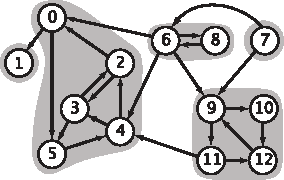
\includegraphics{scc} \hspace{1cm} 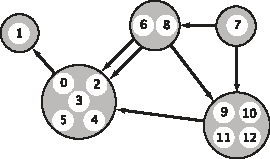
\includegraphics{kernel}}
        \vspace{.4cm}
      \item The SCC of a graph are the same as its reverse, the kernel DAG of a
        graph is the reverse of that of its reverse.
      \end{compactitem}
    \end{minsizebox}};

  \node [heading] (ks) at (-.5\textwidth,-10cm) {~~Kosaraju-Sharir algorithm};
  \node (x) at ($(ks.south west) + (-.2cm, -.2cm)$) {\begin{minsizebox}{19cm}{1.3cm}
      \begin{compactitem}
      \item Step 1: Order nodes s.t.\ if \lstinline{u} is before \lstinline{v}
        and are not in the same SCC, then there is no path from \lstinline{u} to
        \lstinline{v}.
      \item Step 2: Repeated DFS on the graph, following the previous order.
        Each DFS visits a new SCC entirely.
      \end{compactitem}
    \end{minsizebox}};

  \node (p1) [yshift=.3pt,xshift=1cm,fill=algs4red!40,inner sep=0.5cm] at (x.south west) {%
    \begin{minsizebox}{7cm}{4cm}
      \textbf{Why this works.}  If a DFS is started on a node \lstinline{u}, it
      cannot visit nodes that are further in the list if they are not part of
      the same SCC.  Moreover, if a DFS is started on~\lstinline{u}, it means
      that no node of that SCC has been seen in a previous DFS.
    \end{minsizebox} 
    };

    \node[xshift=1cm,fill=algs4red!40,inner sep=0.5cm] (p2) at (p1.north east) {
      \begin{minsizebox}{8cm}{4cm}
        \textbf{How to compute Step 1.}  Compute the reverse postorder of the
        reverse of the graph.\\[3pt]
        \textbf{Proof.} Consider \lstinline{u} appearing before
        \lstinline{v} and assume they are not in the same SCC.  If there were a
        path from \lstinline{u} to \lstinline{v} in \(G\), there would be a path
        from \lstinline{v} to \lstinline{u} in \(G^{\text{rev}}\).  The lemma of
        the previous revision card would imply that \lstinline{v} appears before
        \lstinline{u}, a contradiction.
      \end{minsizebox}
    };

  %% Box
  \draw [algs4red,line width=3pt] [use path=\theframe];

\end{tikzpicture}
\end{document}
